\documentclass[12pt]{article}

\usepackage{answers}
\usepackage{setspace}
\usepackage{graphicx}
\usepackage{enumitem}
\usepackage{multicol}
\usepackage{mathrsfs}
\usepackage[margin=1in]{geometry} 
\usepackage{amsmath,amsthm,amssymb}
\usepackage[ngerman]{babel}

\newcommand{\N}{\mathbb{N}}
\newcommand{\Z}{\mathbb{Z}}
\newcommand{\C}{\mathbb{C}}
\newcommand{\R}{\mathbb{R}}

\DeclareMathOperator{\sech}{sech}
\DeclareMathOperator{\csch}{csch}

\newenvironment{theorem}[2][Theorem]{\begin{trivlist}
		\item[\hskip \labelsep {\bfseries #1}\hskip \labelsep {\bfseries #2.}]}{\end{trivlist}}
\newenvironment{definition}[2][Definition]{\begin{trivlist}
		\item[\hskip \labelsep {\bfseries #1}\hskip \labelsep {\bfseries #2.}]}{\end{trivlist}}
\newenvironment{proposition}[2][Proposition]{\begin{trivlist}
		\item[\hskip \labelsep {\bfseries #1}\hskip \labelsep {\bfseries #2.}]}{\end{trivlist}}
\newenvironment{lemma}[2][Lemma]{\begin{trivlist}
		\item[\hskip \labelsep {\bfseries #1}\hskip \labelsep {\bfseries #2.}]}{\end{trivlist}}
\newenvironment{exercise}[2][Exercise]{\begin{trivlist}
		\item[\hskip \labelsep {\bfseries #1}\hskip \labelsep {\bfseries #2.}]}{\end{trivlist}}
\newenvironment{solution}[2][Solution]{\begin{trivlist}
		\item[\hskip \labelsep {\bfseries #1}]}{\end{trivlist}}
\newenvironment{problem}[2][Problem]{\begin{trivlist}
		\item[\hskip \labelsep {\bfseries #1}\hskip \labelsep {\bfseries #2.}]}{\end{trivlist}}
\newenvironment{question}[2][Question]{\begin{trivlist}
		\item[\hskip \labelsep {\bfseries #1}\hskip \labelsep {\bfseries #2.}]}{\end{trivlist}}
\newenvironment{corollary}[2][Corollary]{\begin{trivlist}
		\item[\hskip \labelsep {\bfseries #1}\hskip \labelsep {\bfseries #2.}]}{\end{trivlist}}

\begin{document}
	\title{Künstliche Intelligenz 2 - Zusammenfassung}
	\author{Michael Gabler}
	\maketitle
	\tableofcontents
	\newpage
	
	\section{Unsicheres Wissen und Schließen}
	Logik benötigt exakte Regeln, die immer wahr sind. Oft nicht gegeben (zu wenig Daten, keine Regeln möglich) $\rightarrow$ wahrscheinlichkeitsbasiertes Entscheiden. Ein Agent benötigt dazu Präferenzen, wie nützlich verschiedene Ziele sind und die Wahrscheinlichkeiten, diese Ziele zu erreichen.\\
	\textbf{Rationalität} = wähle Aktion mit der größten erwarteten Nützlichkeit
	
	\subsection{Wahrscheinlichkeitsrechnung}
	\textbf{unbedingte Wahrscheinlichkeit} $P(A)$\\
	\textbf{Wahrscheinlichkeitsverteilung} $P(Wetter) = (0,7; 0,2; 0,008; 0,02)$\\
	\textbf{Operanden} $\wedge$ = und, $\vee$ = oder\\
	\textbf{Bedingte Wahrscheinlichkeit} wie wahrscheinlich ist $A$ wenn $B$ wahr ist:
	$$P(A|B) = \frac{P(A \wedge B)}{P(B)} \Leftrightarrow P(A \wedge B) = P(A|B) P(B)$$\\
	$P(A \vee B) = P(A) + P(B) - P(A \wedge B)$\\
	\textbf{Apriori-Wahrscheinlichkeit} Wahrscheinlichkeit für ein Ereignis unabhängig von den anderen: $P(X) = \sum_y P(X,y)$ (Marginalization) oder $P(X) = \sum_y P(X|y) P(y)$ (Conditioning)\\
	\textbf{Unabhängige Variablen} Für Variablen, deren Ereignisse unabhängig voneinander eintreten gilt: $P(a|b) = P(a)$\\
	\textbf{Bayes' Theorem} $P(B|A) = \frac{P(A|B) P(B)}{P(A)}$ wird verwendet zur Herleitung nicht bekannter, abhängiger Wahrscheinlichkeiten\\
	\textbf{Naives Theorem von Bayes} Annahme: Symptome $S_i$ untereinander unabhängig (oft nicht gegeben), Vollständigkeit der Diagnosen $D_i$
	$$P(D_i|S_1 \wedge ... \wedge S_m) = \frac{P(D_i) P(S_1|D_i) ... P(S_m|D_i)}{\sum_{j=1}^{n} P(D_j) P(S_1|D_j) ... P(S_m|D_j)} = \alpha P(D_i) P(S_1|D_i) ... P(S_m|D_i)$$
	Dabei ist $\alpha$ eine Normierungskonstante, so dass die Summer aller Wahrscheinlichkeiten 1 ergibt.\\
	\textbf{Numerische Variablen} Annahme: alle Variablen haben diskrete Werte. Kontinuierliche Variablen werden diskretisiert oder Verwendung, wenn Verteilungsfunktion bekannt ist.
	
	\subsection{Probabilistische/Bayessche Netze}
	Theorem von Bayes behandelt alle Symptome als voneinander unabhängig. Probabilistische Netze (gerichtete, azyklische Graphen) stellen Abhängigkeiten dar.\\
	\textit{einfach verbunden}: es gibt nur einen Pfad zu einem Knoten, \textit{mehrfach verbunden}: ex existieren mehrere Pfade zum gleichen Knoten\\
	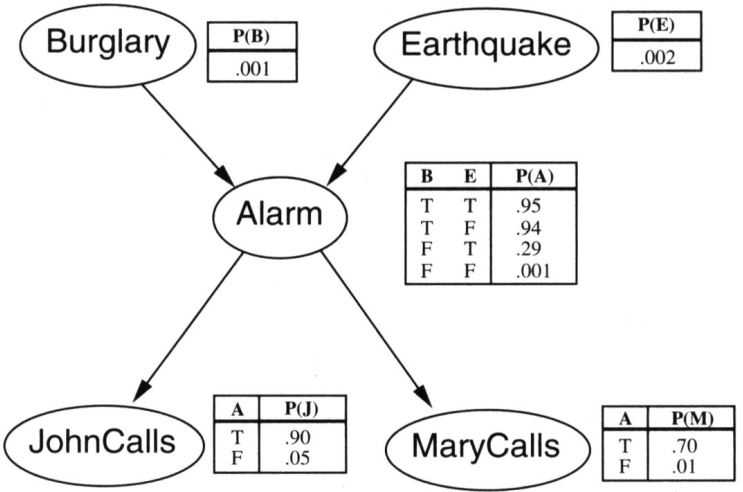
\includegraphics[width=\textwidth]{figures/probabilistisches-netz.JPG}\\
	\textbf{Konstruktion von probabilistischen Netzen}
	\begin{enumerate}
		\item Wähle geeignete Zufallsvariable
		\item Wähle Reihenfolge der Variablen (Wichtig für Größe des Netzes)
		\item Solange Variablen noch nicht im Netz sind:
			\subitem Nimm nächste Variable $X_i$
			\subitem Setze die Eltern von $X_i$ auf eine minimale Menge von bereite im Netz vorhandenen Knoten
			\subitem Definiere die Wahrscheinlichkeitstabelle für $X_i$
	\end{enumerate}
	Es ermöglicht die Wahrscheinlichkeitsberechnung jeder vollständigen Knotenbelegung.\\
	Beispiel: $$P(J \wedge M \wedge A \wedge \bar{B} \wedge \bar{E}) = P(J|A) P(M|A) P(A|\bar{B} \wedge \bar{E}) P(\bar{B}) P(\bar{E}) = 0,9 \cdot 0,7 \cdot 0,0001 \cdot 0,999 \cdot 0,998 = 0,000628$$
	\textbf{Unabhängigkeit} $X$ ist unabhängig von seinen Nichtnachfolgern $Z_{ij}$, wenn seine Eltern $U_i$ bekannt sind (siehe rechts).\\
	$X$ ist unabhängig von allen anderen Knoten, wenn seine Eltern $U_i$, seine Kinder $Y_i$ und deren andere Eltern $Z_{ij}$ bekannt sind $\Rightarrow$ Markov blanket (siehe links)\\
	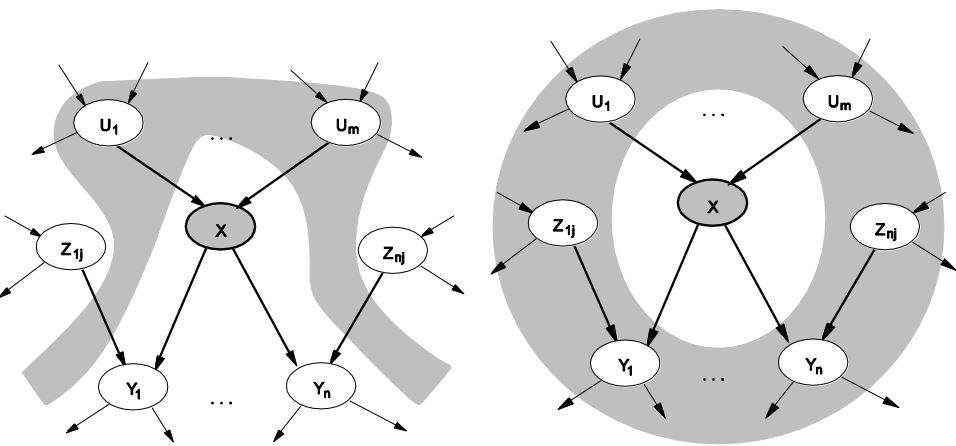
\includegraphics[width=\textwidth]{figures/markov-blanket.JPG}
	\textbf{Enumerate-Joint-Ask} Berechnung von nicht vollständigen Knotenbelegungen $\rightarrow$ bilde Summe über unbekannte Möglichkeiten: $$P(B|J \wedge M) = \alpha P(B,J,M) = \alpha \sum_e \sum_a P(B \wedge e \wedge a \wedge J \wedge M)$$
	$\Rightarrow$ Komplexität für $n$ boolsche Variablen: $O(n2^n)$\\
	\textbf{Verbesserungen} Speichern von Berechnungen, Verschiebung von Termen vor die Summe, Irrelevante Variablen die 1 ergeben erkennen und eliminieren, Zusammenfassung von Knoten in mehrfach verbundenen Netzen\\
	\textbf{Stochastische Simulation} Führe mehrere Simulationsläufe mit Zufallswerten durch und berechne aus den Häufigkeiten die Wahrscheinlichkeiten.
	\begin{itemize}
		\item Direct Sampling: wähle Werte in topologischer Reihenfolge der Wahrscheinlichkeitstabelle entsprechend $\rightarrow$ erfordert viele Läufe für seltene Ereignisse
		\item Rejection Sampling: wie Direct Sampling, aber nicht relevante Läufe werden ignoriert
		\item Likelihood Weighting: setze interessante Werte und gewichte entsprechend der Wahrscheinlichkeitstabellen $\rightarrow$ effizient, kann aber nicht alles gleichzeitig berechnen
		\item Markov Chain Monte Carlo (MCMC): wähle Wertebelegung entsprechend der Vorgaben, restliche Knoten werden zufällig entsprechend ihrer Markov Blanket gewählt
	\end{itemize}
	\textbf{Berechnung der wahrscheinlichsten Sequenz} Wahrscheinlichkeiten für Zustände in Abhängigkeit einer Variable gegeben, Wahrscheinlichkeit für Auftreten des Folgezustandes gegeben. Berechne wahrscheinlichste Sequenz durch durchrechnen.\\
	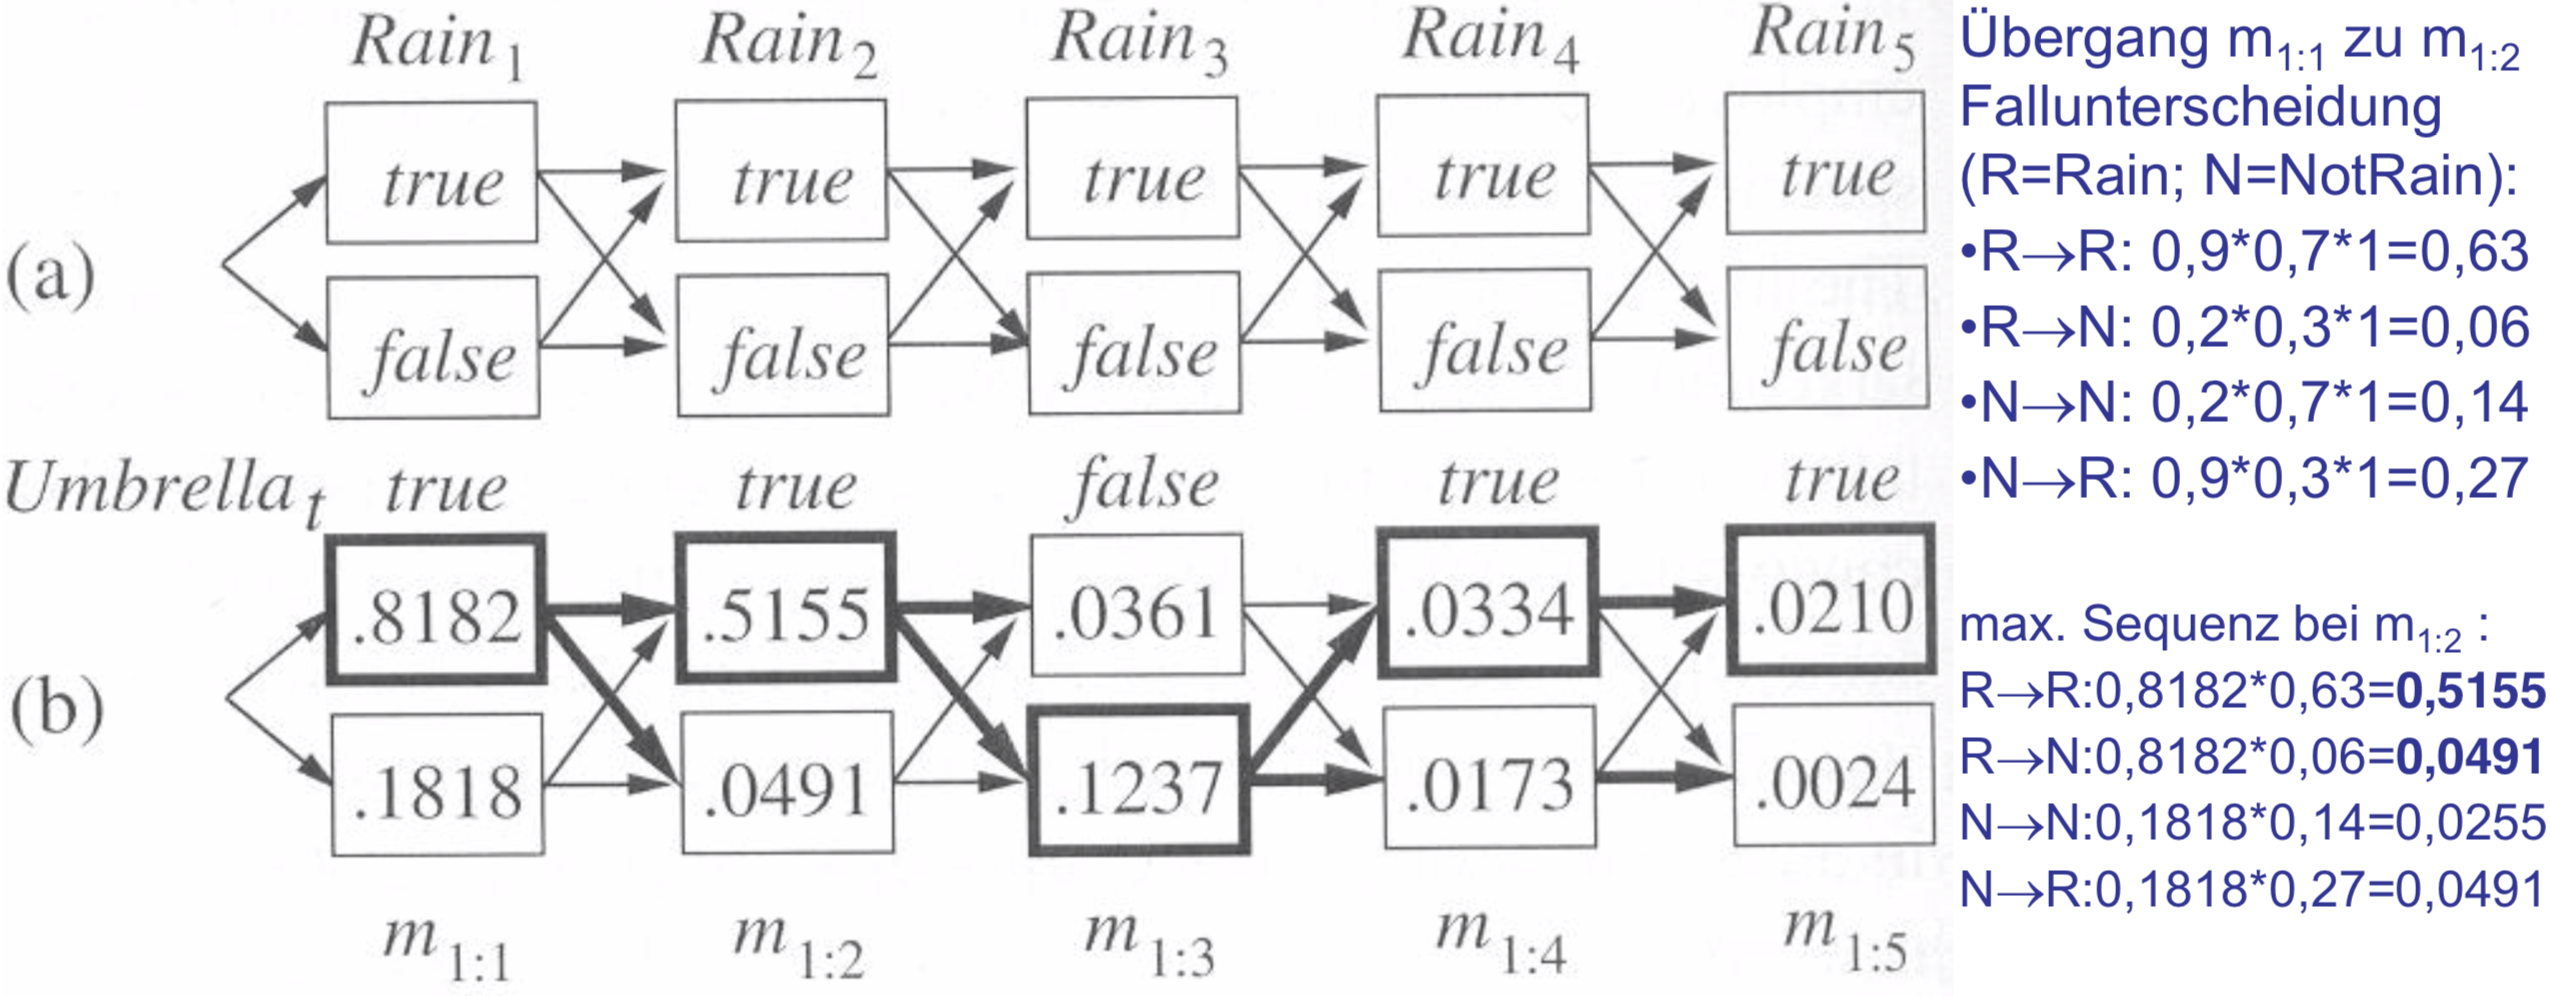
\includegraphics[width=\textwidth]{figures/wahrscheinlichste-sequenz.png}\\
	\textbf{Hidden Markov Model} Reduktion aller Variable auf eine einzige, die alle Zustände abbildet $\rightarrow$ wird zur Abbildung von Phonemen (Lauten) auf Wörter verwendet\\
	\textbf{Kalman Filter} Schätzung des Zustandes eines physischen Systems anhand verrauschter Beobachtungen (z.B. Flugzeuge auf Radarschirm)\\
	\textbf{Viterbi Algorithmus} rekursives Vorgehen
	
	\subsection{Entscheiden}
	\textbf{Erwartete Nützlichkeit} Ziel einer Entscheidung sollte die Maximierung der erwarteten Nützlichkeit $EU$ sein. Diese berechnet sich unter der Vorbedingung $E$ für eine Aktion $A$ mit $i$ verschiedenen Ergebnissen wie folgt: $EU(A|E) = \sum_i P(Ergebnis_i(A)|E, Tue(A)) U(Ergebnis_i(A))$ mit $U$ als Nützlichkeit\\
	\textbf{Axiome der Nützlichkeitstheorie}
	\begin{itemize}
		\item Reihenfolge: $(A \succ B) \vee (B \succ A) \vee (A \sim B)$
		\item Transitivität: $(A \succ B) \wedge (B \succ C) \Rightarrow (A \succ C)$
		\item Kontinuität: $A \succ B \succ C$ Agent ist unsicher, wenn er $B$ sicher bekommt, $A$ aber nur mit Wahrscheinlichkeit $p$ und $C$ mit $1-p$
		\item Ersetzbarkeit: gleiche Entscheidung für komplexere Lotterien, die $A$ und $B$ enthalten wie zwischen nur $A$ und $B$
		\item Monotonie: zwei Lotterien mit der Nützlichkeit $A$ und $B$. Wenn $A$ besser als $B$, dann muss auch andere Lotterie bevorzugt werden, die $A$ mit höherer Wahrscheinlichkeit nutzt
		\item Zerlegbarkeit: Komplexe Lotterien können vereinfacht werden, da der Agent keine Lotterie bevorzugen sollte, nur weil er mehr Wahlmöglichkeiten hat
	\end{itemize}
	\textbf{Probleme} Beste Wahrscheinlichkeiten oft überschätzt; Mensch entscheidet nicht rational\\
	strikt dominant: in jedem Attribut besser; stochastisch dominant: besser für jedes Wahrscheinlichkeitsniveau\\
	\textbf{Entscheidungsnetze} Erweiterung von probabilistischen Netzen um Entscheidungs- und Nützlichkeitsknoten. $\rightarrow$ Entscheidungsknoten beeinflussen die Zufallsvariablen und damit die Nützlichkeit. Vorgehen zur Auswertung:
	\begin{enumerate}
		\item Setze Zufallsvariablen entsprechend dem aktuellen Zustand
		\item Für jede mögliche Aktion des Entscheidungsknotens:
			\subitem Setze den Entscheidungsknoten auf diesen Wert
			\subitem Berechne Wahrscheinlichkeiten der Eltern-Knoten des Nützlichkeitsknoten mit einem Inferenz-Algorithmus für probabilistische Werte
			\subitem Berechne Nützlichkeit der Aktion
		\item Wähle Aktion mit größter Nützlichkeit
	\end{enumerate}
	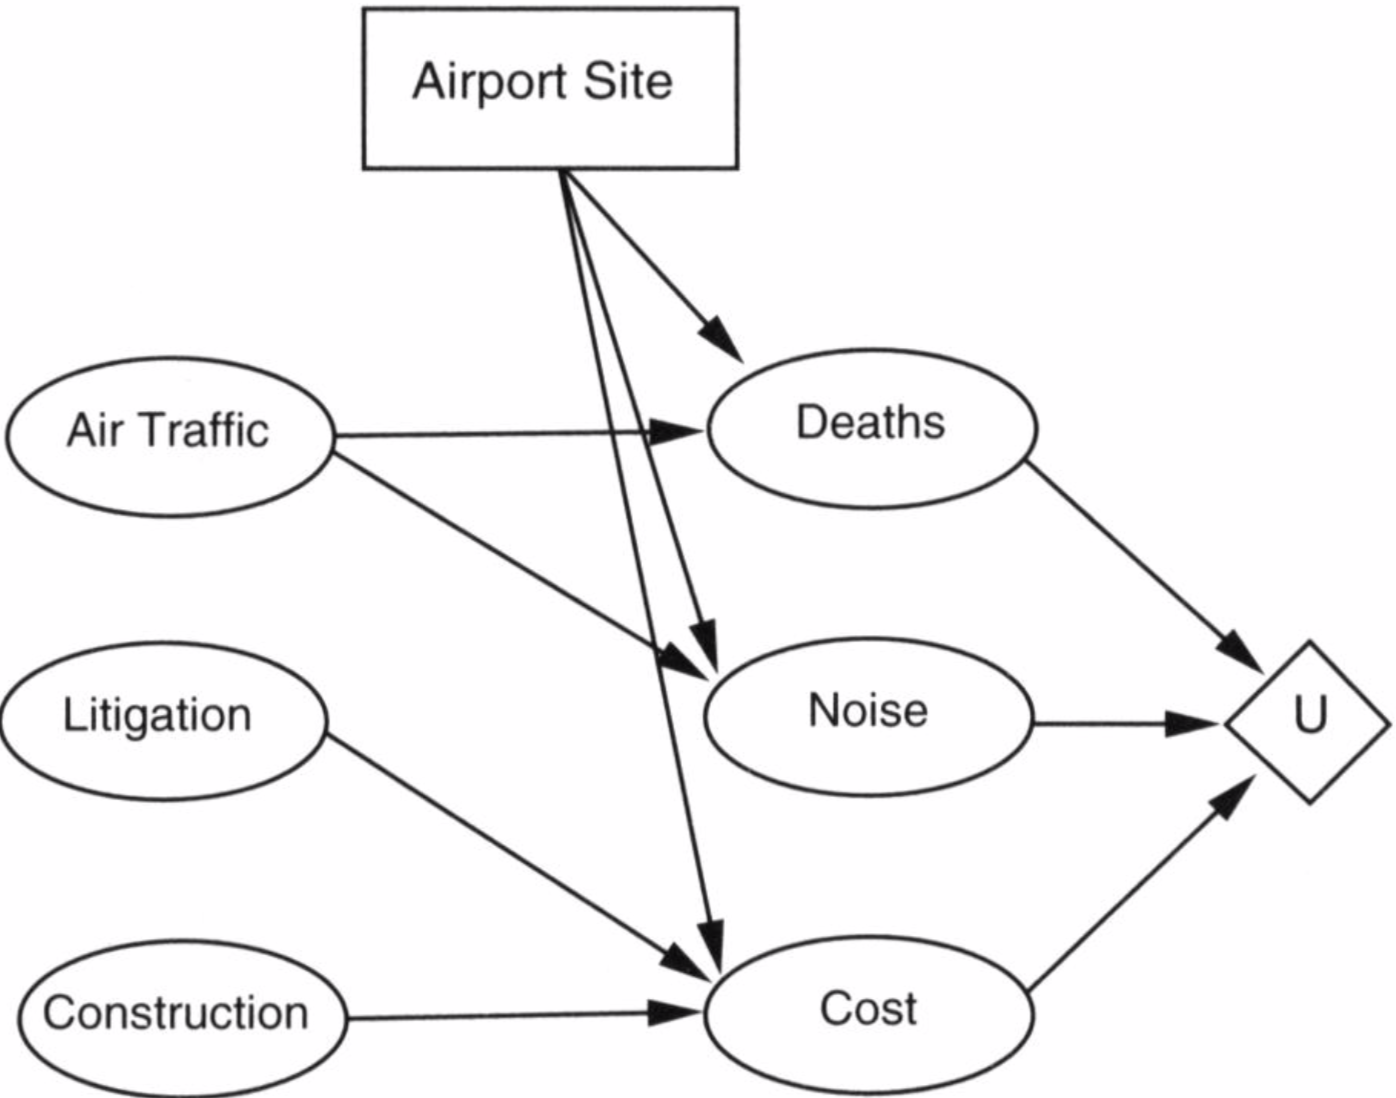
\includegraphics[width=0.5\textwidth]{figures/entscheidungsnetz.png}\\
	Bewertung der Nützlichkeit ist genauer mit mehr Informationen. Nützlichkeit der Information ist immer positiv, nicht additiv und kann berechnet werden.
	
	\section{Lernen}
	Lernende Agenten haben \textbf{Verhaltenskomponente} (Problemlöser), \textbf{Lernkomponente} (Verbesserung der Verhaltenskomponente), \textbf{Kritikkomponente} (Bewertung des Verhaltens) und einen \textbf{Problemgenerator} (Exploration). Lernen kann dabei als Lernen der Repräsentation einer Funktion betrachtet werden.\\
	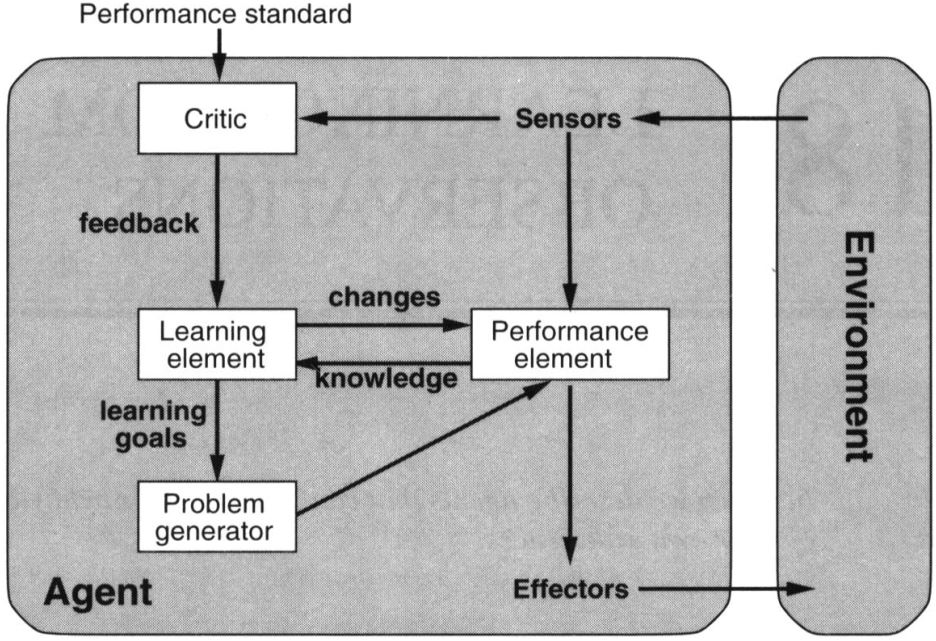
\includegraphics[width=\linewidth]{figures/lernender-agent.JPG}\\
	\textbf{Lernarten}
	\begin{enumerate}
		\item Geführtes Lernen (Supervised learning)
		\item Verstärkungslernen (reinforcement learning)
		\item Ungeführtes Lernen (unsupervised learning)
		\item Teilgeführtes Lernen (semi-supervised learning)
	\end{enumerate}
	\textbf{Lernen einer Funktion} Gegeben Ausgaben einer Funktion, die approximiert werden soll. Aufteilung in Trainingsmenge und Testmenge. Bei \textbf{endlicher} Ausgabemenge $\Rightarrow$ \textbf{Klassifikation}, bei \textbf{kontinuierlicher} Ausgabe $\Rightarrow$ \textbf{Regession}\\
	\textbf{Auswahl verfügbarer Hypothesen} (gelernte Funktionen): bevorzuge einfache Hypothese (Ockham's razor) $\Rightarrow$ Präferenzannahme (\textbf{Bias})\\
	\textbf{Entropie}: Informationsmaß für die Unsicherheit einer Zufallsvariable. Wie viel Bit werden benötigt, um die Zustände zu repräsentieren? (z.B. Münze werfen $\rightarrow$ 1 Bit, 4-seitiger Würfel $\rightarrow$ 2 Bit, aber Münze mit 99 \% Wahrscheinlichkeit für Zahl $\rightarrow > 0$). Allgemein: Entropie $H$ der Zufallsvariablen $V$, deren Werte $v_k$ sind
	$$H(V) = \sum_k P(v_k) \log_2 \frac{1}{P(v_k)} = - \sum_k P(v_k) \log_2 P(v_k)$$
	Damit ergibt sich eine Entropie $B$ für boolsche Variablen, die mit der Wahrscheinlichkeit $q$ wahr sind: $B(q) = - (q \log_2 q + (1-q) \log_2 (1-q))$.\\
	\textbf{Overfitting} beschreibt das zu starke Anpassen eines Lernmodells an die Testdaten, wodurch die Klassifikation auf realen Daten schlecht funktioniert.\\
	\textbf{Pruning} Entfernen irrelevanter Attribute (zufällige Aufteilung) $\rightarrow$ Chi-Quadrat-Test\\
	\textbf{Cross-Validation} Überprüfe Bewertungsgenauigkeit mit unabhängigem Testset an Daten (reservierter Teil der Trainingsdaten) $\rightarrow$ k-fold Cross Validation reserviert für jeden der $k$ Trainigsdurchgänge $\frac{1}{k}$ der Trainingsdaten als Testdaten\\
	\textbf{Loss Function} (Verlustfunktion) ist ein Maß dafür, wie viele Fehler das aktuellen Modell bei der Klassifizierung macht (kann z.B. nach Schwere des Fehlers gewichtet werden)\\
	\textbf{Lernrate $\alpha$} Beginne mit zufälliger Belegung der Variablen und subtrahiere die Lossfunktion, multipliziert mit einem Faktor $\alpha$ (konstant oder schrittweise verkleinern, z.B. durch Gradientenberechnung), der Lernrate.\\
	\textbf{Schwellwertfunktion} $h_w(x) = Schwellwert(w \cdot x)$ Klassifikation über Schwellwert\\
	\textbf{Sigmoid-Funktion} Schwellwertfunktion nicht ableitbar, deshalb ersetzen durch Sigmoid-Funktion/logistische Funktion: $sig(x) = \frac{1}{1 + e^{-x}}$\\
	\textbf{Ensemble Lernen} Mehrere Hypothesen aufstellen und diese per Mehrheit abstimmen lassen. Hypothesen können durch unterschiedliche Gewichtung der Beispiele gelernt werden $\rightarrow$ Boosting
	
	\subsection{Lernen von Entscheidungsbäumen}
	Für den Mensch einfach verständlich, Ausgabe ist Ja/Nein-Entscheidung (boolean). Für $n$ verschiedene boolsche Eingabewerte existieren $2^{2^n}$ mögliche boolsche Funktionen.\\
	\textbf{Entscheidungsbaum mit Trainingsbeispielen}\\
	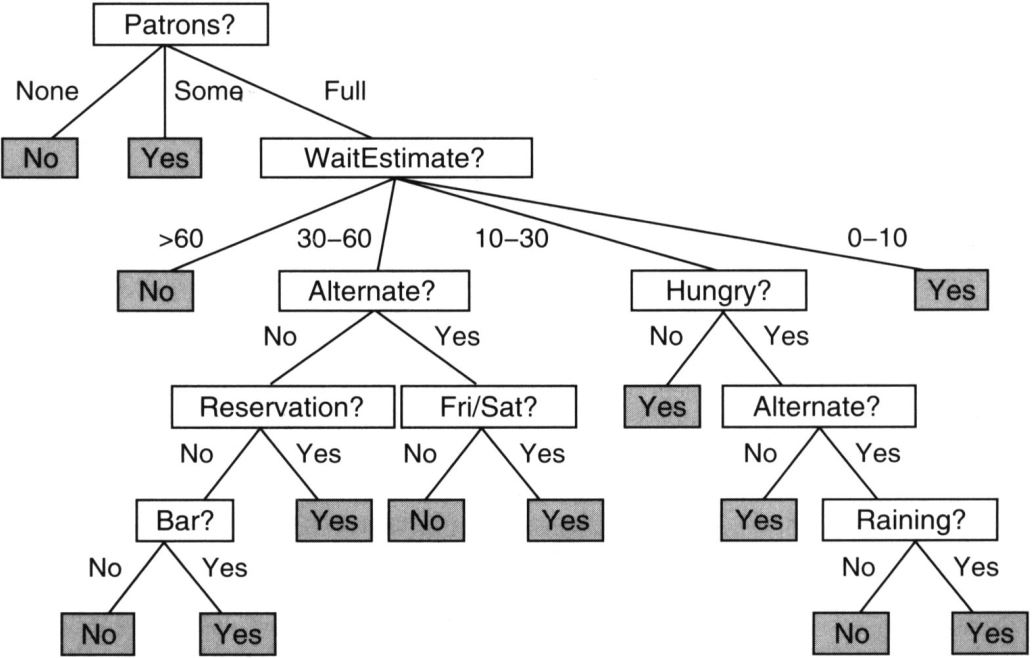
\includegraphics[width=0.5\linewidth]{figures/entscheidungsbaum.JPG}
	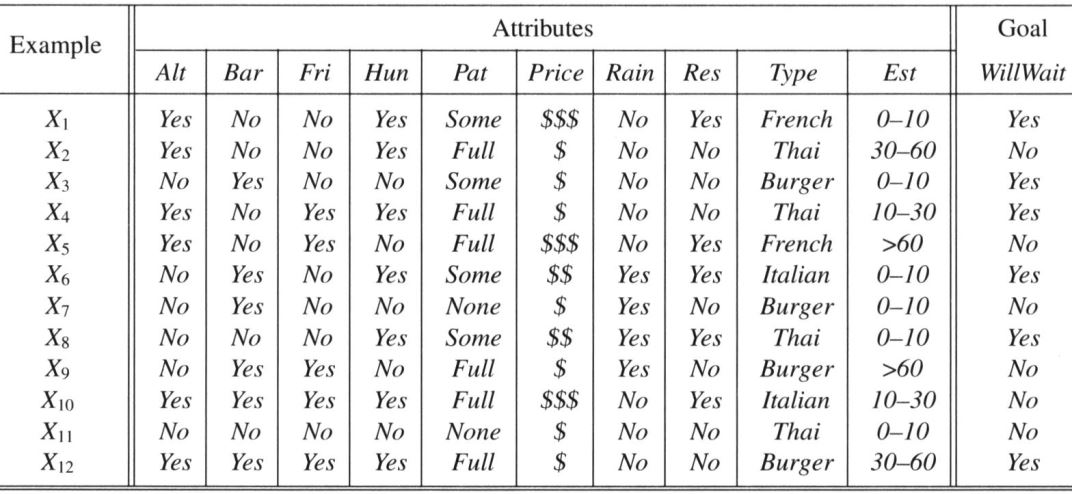
\includegraphics[width=0.5\linewidth]{figures/entscheidungsbaum-trainingsbeispiele.JPG}\\
	Für den Aufbau des Baums wähle Attribut aus der Trainingsmenge, das die meisten Zielzustände exakt vorhersagen kann/bedingt. Fahre rekursiv fort. Beispiel: für alle $Patrons = Some \Rightarrow WillWait = Yes$\\
	\textbf{Entropie in Entscheidungsbäumen} Für Entscheidungsbäume mit $p$ positiven und $n$ negativen Trainingsdatensätzen ergibt sich: $H(Ziel) = B(\frac{p}{p+n})$. Für ein Attribut $A$ mit $d$ verschiedenen Werten ergibt sich dann eine Entropie von: $Remainder(A) = \sum_{k=1}^{d} \frac{p_k + n_k}{p+n} B(\frac{p_k}{p_k + n_k})$. Die erwartete Entropiereduktion ist er Informationsgewinn des Attributs $A$ und beschreibt damit dessen Wichtigkeit (Entscheidungskriterium für bestes Attribut): $Gain(A) = B(\frac{p}{p+n}) - Remainder(A)$\\
	\textbf{Probleme} Unvollständige Daten $\rightarrow$ Werte schätzen, Attribute mit vielen Werten $\rightarrow$ Pruning\\
	
	\subsection{Lernen von Entscheidungslisten (Regeln)}
	\textbf{Greedy-Algorithmus} Eingabe: alle Beispiele $B$, Ausgabe: Entscheidungsliste $E$, leer initialisiert
	\begin{itemize}
		\item Wenn $B$ leer dann return $E$
		\item Suche Regel $R$, die möglichst viele Beispiele $B_R$ löst
		\item Wenn Regel gefunden $E \leftarrow append(E, R)$, $B \leftarrow B \backslash B_R$, sonst return Error
	\end{itemize}

	\subsection{Lineare Regression}
	Lernen von linearen Geradengleichungen, d.h. suche Vektor $w = [w_0, w_1]^T$ für $h_w(x) = w_1 x + w_0$. $\Rightarrow$ binäre Klassifikation möglich mit Schwellwertfunktion\\
	\textbf{$L_2$-Loss} Berechnung der quadratischen Differenz zwischen vorhergesagtem Wert $(x_j, h_w(x_j))$ und erwartetem Ergebnis $(x_j, y_j)$ bei $N$ Datenpunkten:
	$$Verlust(h_w) = \sum_{j=1}^{N} L_2(y_j, h_w(x_j)) = \sum_{j=1}^{N} (y_j - h_w(x_j))^2 = \sum_{j=1}^{N} (y_j - (w_1 x_j + w_0))^2$$
	Die Summe der Fehler ist minimal, wenn die Ableitungen nach $w_0$ und $w_1$ null sind. Daraus ergibt sich für $w$:
	$$w_1 = \frac{N(\sum x_j y_j) - (\sum x_j)(\sum y_j)}{N(\sum x_j^2)-(\sum x_j)^2}, w_0 = \frac{\sum y_j - w_1 (\sum x_j)}{N}$$
	$\Rightarrow$ schwer berechenbar, daher Hill-Climbing mit Gradientenabstieg
	
	\subsection{Support Vector Machine (SVM)}
	Linear trennende Hyperebene in höherdimensionalem Raum mit zusätzlichen Attributen generiert aus den vorhandenen (z.B. räumliche Verschiebung von 2D-Punkten) $\Rightarrow$ größerer Rechenaufwand als bei Deep Learning\\
	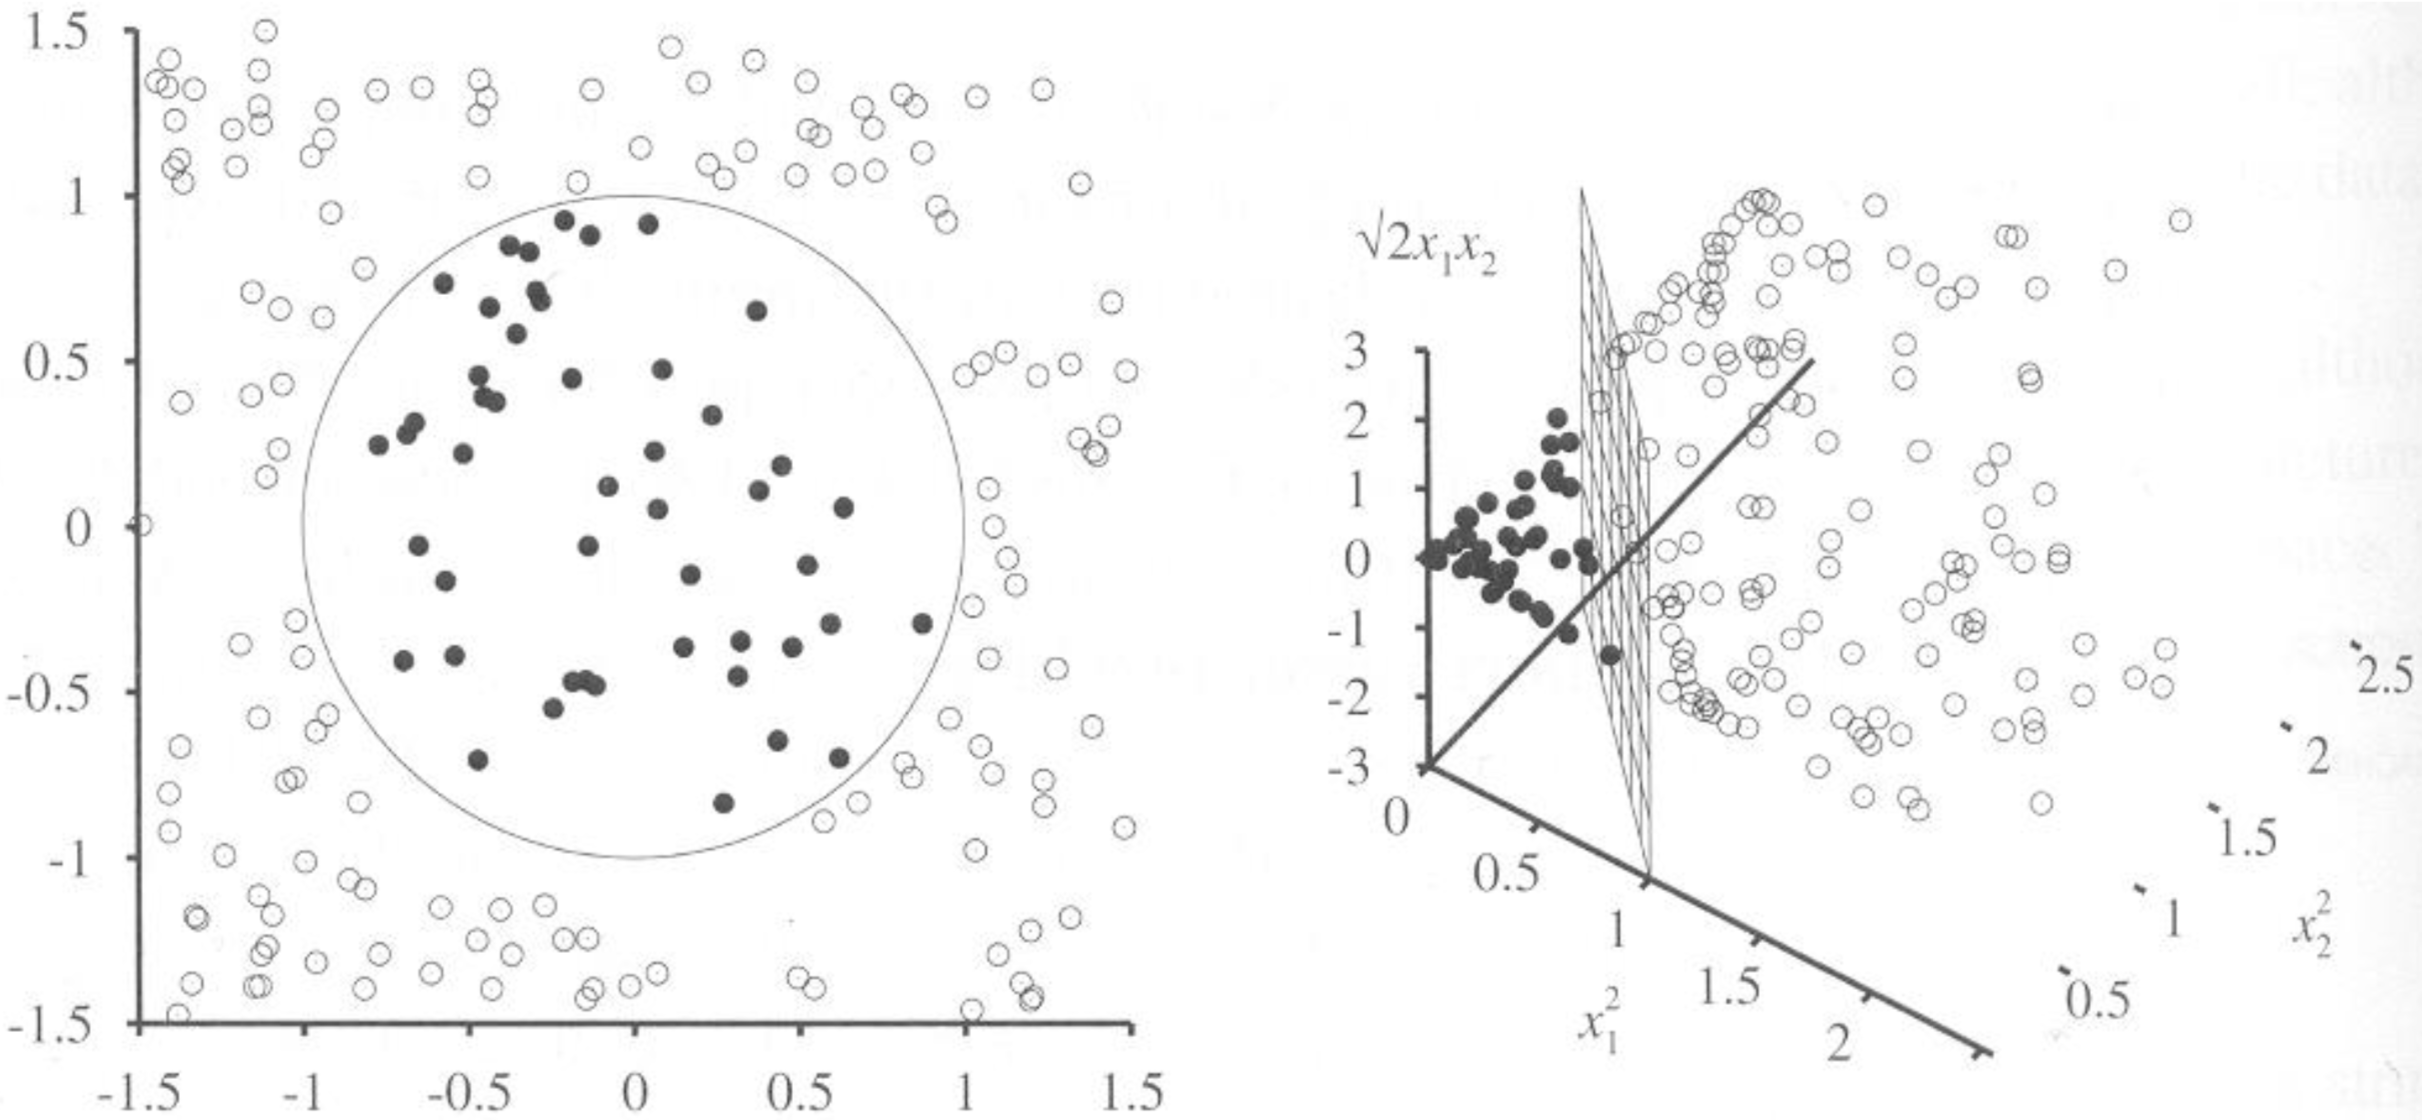
\includegraphics[width=\linewidth]{figures/support-vector-machine.png}
	
	\subsection{Lernen in Bayesschen Netzen}
	\begin{enumerate}
		\item Bekannte Netzstruktur, beobachtbare Variablen $\rightarrow$ Update der Wahrscheinlichkeitstabellen
		\item Bekannte Netzstruktur, teilweise nicht beobachtbare Variablen $\rightarrow$ EM-Algorithmus
		\item Unbekannte Netzstruktur, beobachtbare Variablen $\rightarrow$ Suchproblem
		\item Unbekannte Netzstruktur, teilweise nicht beobachtbare Variablen $\rightarrow$ offenes Forschungsproblem
	\end{enumerate}
	Berechne die Wahrscheinlichkeit für gegebene Hypothesen $H_i$ unter gegebenen Beobachtungen $B_i$ (z.B. welche Tüte Bonbons (5 Arten) wurde gekauft, wenn nacheinander mehrere Bonbons gezogen werden): $P(H_i|B) = P(B|H_i) P(H_i) \Rightarrow P(B|H_i) = P(B_1|H_i) ... P(B_n|H_i)$\\
	\textbf{Maximum a Posteriori} Benutze in letzter Berechnung nur wahrscheinlichste Hypothese\\
	\textbf{Maximum Likelihood} Ignoriere in erster Berechnung die a priori Wahrscheinlichkeiten $P(H_i)$ der Hypothesen (oft ungenau).\\
	\textbf{Expectation-Maximation (EM) Algorithmus} Gegeben: Punktemenge in $n$-dimensionalem Raum (Trainingsdaten); Gesucht: eine Menge von $c$ Clustern (Klassifikation)
	\begin{itemize}
		\item Initialisierung: wähle zufällig $c$ Clusterzentren
		\item Expectation: Ordne jeden Punkt dem nächstgelegenen Clusterzentrum zu
		\item Maximation: Berechne aufgrund der Cluster-Punkte dessen Zentrum neu
		\item Terminierung: wiederhole E- und M-Schritt, bis kein Punkt seine Clusterzugehörigkeit ändert $\rightarrow$ keine Verbesserung mehr
	\end{itemize}
	
	\subsection{Reinforcement Learning}
	Lernen durch Feedback. Agent lernt, in dem er zu seinen Aktionen zu einem definierten Zeitpunkt ein Feedback bekommt (gut oder schlecht).
	\begin{itemize}
		\item Nützlichkeitsbasiert: Agent lernt Nützlichkeit von Zuständen zur Aktionsauswahl
		\item Q-Learning: Agent lernt Aktion-Wert-Funktionen
		\item Reflexartig: Agent lernt Politik, die Zustände auf Aktionen abbildet
		\item Passiv: Politik steht fest $\rightarrow$ lernt Nützlichkeit der Zustände
	\end{itemize}
	\textbf{Erkundungspolitik} wenig erkundete Pfade bekommen belohnungsabhängige Verstärkung, die mit häufigeren Durchläufen abnimmt.\\
	\textbf{Q-Lernen} $Q(a,s)$ = Wert der Aktion $a$ im Zustand $s \Rightarrow U(s) = \max_a Q(a,s)$ Nützlichkeit eines Zustandes ist die größte Nützlichkeit einer der möglichen Aktionen. Stelle Tabelle mit Zustandsübergängen dar und deren Nützlichkeiten (z.B. Roboter versucht von einem Raum in einen anderen gelangen). Das Ziel hat höchste Nützlichkeit. Starte in jedem Durchgang in beliebigem Zustand (z.B. in beliebigem Raum) und wähle zufällige Aktion. Berechne Nützlichkeit für Zustand:
	$$Q(s,a) = R(s,a) + \gamma \max_{a'} Q(s',a')$$
	
	\subsection{Neuronale Netze}
	Neuronale Netze entstehen durch die Verknüpfung mehrerer Schichten von künstlichen Neuronen, wobei jedes Neuron als Eingabe die Ausgaben aller Neuronen der vorherigen Schicht erhält (fully-connected).\\
	\textbf{Perceptron} (= künstliches Neuron) stellt lineare Trennung (binäre Klassifikation) dar. Kann Funktionen AND, OR und NOT lernen, nicht aber XOR.\\
	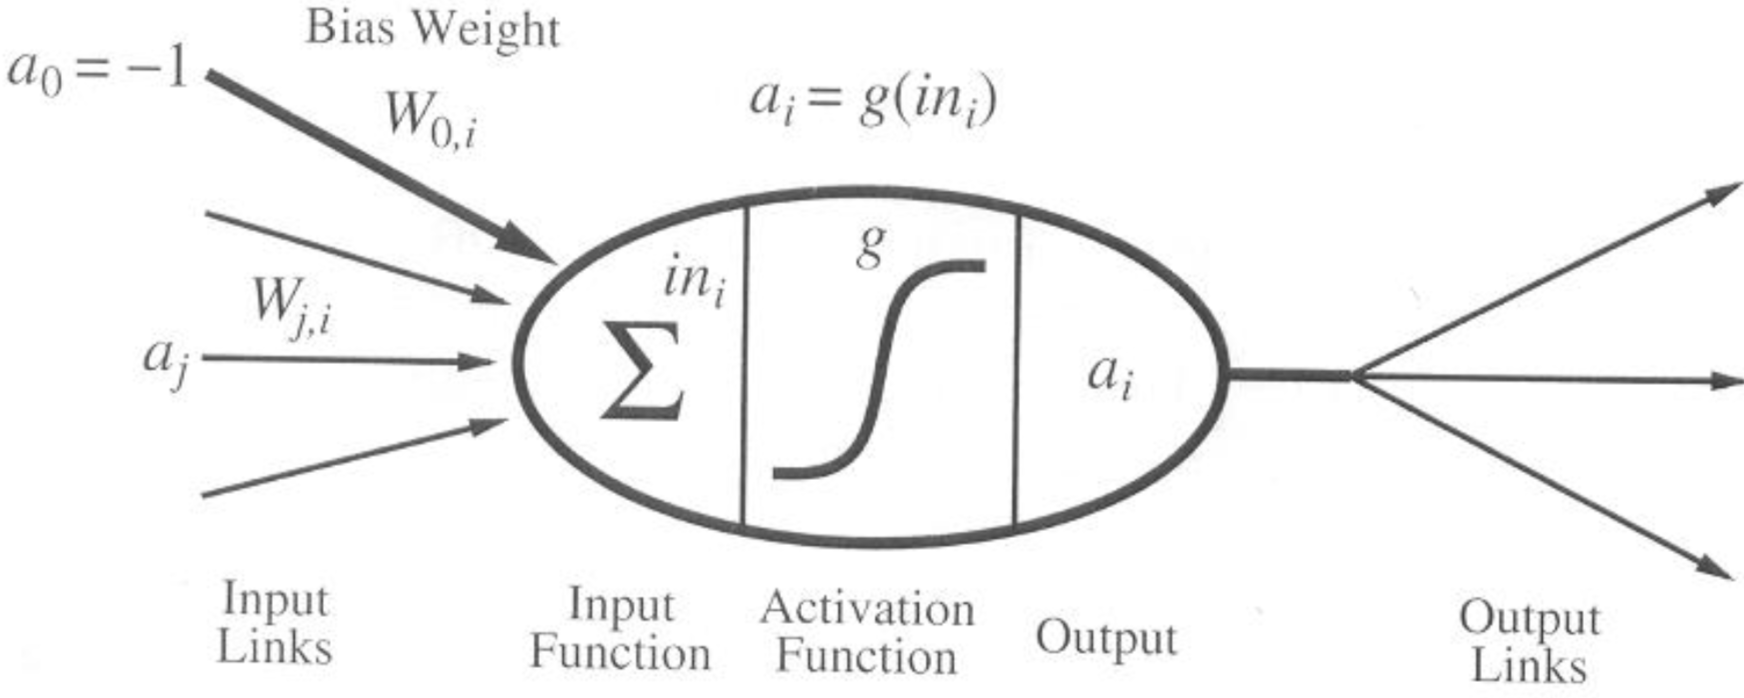
\includegraphics[width=\linewidth]{figures/perceptron.png}\\
	mit Inputs $a_j$ gewichtet mit $W_{ji}$ (ergeben zusammen die Gewichtsmatrix $W$), Outputs $a_i$ und der Aktivierungsfunktion $g$ mit der der Output berechnet wird.\\
	\textbf{Bias} ist der Input eines Perceptrons, der immer konstant bleibt (meist 1) damit das Perceptron auch bei schwachem Input nicht abgeschaltet wird.\\
	\textbf{Aktivierungsfunktionen} typisch sind:
	\begin{itemize}
		\item Stufenfunktion: $g(x) = x < 0 \rightarrow 0, x > 0 \rightarrow 1$ (nicht differenzierbar)
		\item Sigmoidfunktion: $g(x) = \frac{1}{1 + e^{-x}}$ (siehe Einleitung Lernen)
		\item ReLU (Rectified Linear Unit): $g(x) = x < 0 \rightarrow 0, x > 0 \rightarrow x$ (nicht differenzierbar für $x=0$)
		\item Tangenz hyperbolicus: $g(x) = tanh(x)$
		\item Softmax: Abbildung eines Vektors in Werte zwischen 0 und 1 mit Summe 1 (z.B. für Ausgabelayer)
	\end{itemize}
	\textbf{Rückpropagierung} Fehler (z.B. quadratische Abweichung von erwartetem Wert $\rightarrow$ Loss-Funktion) wird entsprechend der Gewichte auf Vorgängerknoten verteilt\\
	\textbf{Berechnung der Ausgabe}
	$$Ausgabe_{Schicht(x)} = g(W \cdot Eingabe_{Schicht(x)}) = Eingabe_{Schicht(x+1)}$$
	\textbf{Verteilung des Fehlers}
	$$Fehler_{Schicht(x-1)} = W^T \cdot Fehler_{Schicht(x)}$$
	Änderung der Gewichte über Gradient Descent $w_{jk} \leftarrow w_{jk} - \alpha \frac{dE}{dw_{jk}}$ mit $E$ als Loss-Funktion\\
	\textbf{Datenvorverarbeitung} Inputs zwischen 0 und 1, da hohe Werte niedrige Gradienten erzeugen, Bilder können rotiert, gespiegelt, zugeschnitten, etc. werden um mehr Trainingsdaten zu generieren.\\
	\textbf{Netzvorbereitung} zufällige Vorbelegung der Gewichte (nicht symmetrisch) $\Rightarrow$ Pre-Training: wenn möglich Gewichte eines bereits trainierten Netzes für ähnliches Problem verwenden\\
	\textbf{Overfitting} kann durch kleine Netzgröße (nicht so ausdrucksstark), Dropout (ignorieren einiger Knoten für einen Lerndurchgang)\\
	\textbf{Typen von Schichten}
	\begin{itemize}
		\item Fully Connected (FC): besteht aus mehreren Perceptrons (s.o.)
		\item Convolutional Neural Networks (CNN): Für Bilderkennung, Gewichtungsmatrix über Input verschieben und gewichtete, aufsummierte Werte in Outputmatrix schreiben
		\item Polling Layer: Verkleinerung von Inputmatrizen durch z.B. Max-Funktion einer Submatrix
	\end{itemize}
	\textbf{Multi-Klassen Klassifizierung} über $K$ Diskrimianzfunktionen für $K$ Klassen. Dabei gibt immer eine Funktion für einen bestimmten Bereich/Klasse den höchsten Wert zurück.\\
	\textbf{Vanishing Problem} Tiefe Netze lernen sehr langsam, da das Änderungsgewicht pro Schicht mit Faktor < 1 multipliziert wird (Ableitung Aktivierungsfunktion). Kann umgangen werden durch ReLU (Ableitung konstant 1 für positive Zahlen)\\
	\textbf{Recurrent Neural Networks} für die Verarbeitung von sequenziellen Daten (variable Ein-/Ausgabe) z.B. für OCR oder Sprachverarbeitung\\
	\textbf{CTC-Algorithmus} Berechne die Wahrscheinlichkeit einer Sequenz durch Aufsummieren aller möglichen Pfade (links) oder dynamisches Programmieren (rechts)\\
	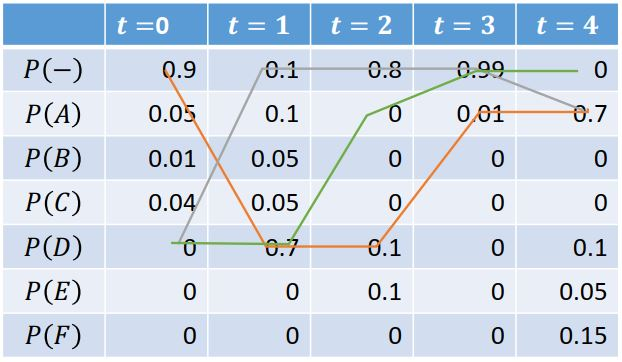
\includegraphics[width=0.5\linewidth]{figures/ctc-pfade.JPG}
	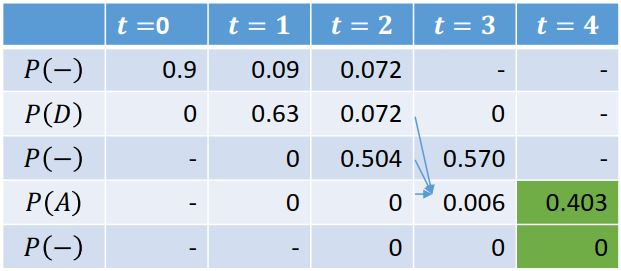
\includegraphics[width=0.5\linewidth]{figures/ctc-dynamisch.JPG}\\
	\textbf{Adversial Examples} Manipulierte Inputdaten, die für den Menschen noch gut erkennbar sind (kein merklicher Unterschied zu Original), von einem DNN jedoch falsch klassifiziert werden. Bild wird mit Rauschen addiert, welches auf das Netz trainiert ist. Gegenmaßnahmen:
	\begin{itemize}
		\item Trainiere Netz mit Adversial Examples (richtige Klassifikation)
		\item Mehrere unterschiedliche Technologien zur Klassifikation einsetzen
		\item DeepCloak entfernen von unnötigen Features, die ausgenutzt werden könnten
	\end{itemize}
	
\end{document}
